\section{Discussion}
\label{sec:discussion}

\subsection{What is different about a millimetre technosignature search}
\label{sec:mmdifferent}

The most transferable result of this experiment is not the non-detection but
a measurement of what limits a carrier search at these wavelengths. It is not
depth: the power a transmitter must radiate to cross the threshold here is a median
$\EirpNinetySysMedA$\,W per system, and more power buys nothing at a
frequency the archive never tuned to or never returned to. What limits the
search is that inherited coverage. Molecular-line confusion is a different
matter: it costs bandwidth, and it decides how a crossing is disposed of once
one is found.

\emph{Line emission, and not interference, is the astrophysical false
positive here.}
Catalogued molecular transitions, almost all of them carbon monoxide, account
for \EvNAttrQp{} of the \EvNCrossQp{} crossings in quality-passing data, and
no crossing in this survey is attributed to interference
(Appendix~\ref{app:rfi}). \LnAttrSupp{} of those attributions carry support
beyond the frequency match -- a second transition of the same species,
catalogued gas on the sightline, or the crossing's own recurrence -- while
\LnAttrCoincWord{} rest on the coincidence alone, which leaves them
consistent with molecular emission rather than identified as it. The
attributed crossings include the strongest events in the quality-passing
data, but they are
not the commonest: of the \EvNUnattrQp{} unattributed crossings the \CeObs{}
of the primary census are no more numerous than the control positions of
their own fields predict
(\S\ref{sec:trigunif}), so chance at a trigger of \StageNullTrig{} is enough
to account for most crossings by number while line emission accounts for the
ones that stand out.
\DiscFpWin{} of the \DiscFpOfFlags{} windows that reached the spatial stage
are disc or foreground carbon monoxide, all but one the resolved disc of
$\beta$~Pictoris and the exception a cloud along the sightline to
HD~48370. The remedy that works is a velocity-space mask evaluated in each star's
own rest frame, and \S\ref{sec:bpicval} gives what it costs in
bandwidth.

\emph{Spatially extended emission is the second discriminant, and it has no
analogue at centimetre wavelengths.} A line filling the primary beam raises
the star and the control annulus together instead of cancelling, so the
spatial statistic loses power exactly where circumstellar gas is brightest.
$\beta$~Pictoris shows the benign face, its circumstellar carbon monoxide
recovered blind (\S\ref{sec:bpicval}); HD~48370 shows the other. Its
emission is foreground cloud rather than a disc
(Appendix~\ref{app:linemask}), it lies near a band edge, and that one window
contributes \VnEdgeDomPct{} per cent of every near-edge threshold exceedance
in the survey. Pooled, the near-edge rate is $\times\VnEdgeRatio$ the
interior rate; without that window it is $\times\VnEdgeNoDomRatio$, and on a
held-out half $\times\VnEdgeHalfCleanRatio$
($\pv{\VnEdgeHalfCleanP}$). What looked like a
property of band edges is one foreground cloud, so no edge correction is
applied to any limit.

\emph{The channelisation is inherited.} In \ScCoarseNoDrift{} of the
\NWinB{} coarse-channel windows every drift in the grid stays inside one channel over a
whole track and in \EtaDriftBHi{} more it crosses barely one; none of them
can distinguish a drifting carrier from a stationary one, which is why the
carrier search rests on the \NWinA{} fine-channel windows. The widths on offer here run from \SzChanFinestKHz\,kHz to
\SzChanWidestMHz\,MHz, about \SzChanDexSurvey{} orders of magnitude. Set
beside the \SzChanLitHz\,Hz channels of centimetre-band carrier searches the
range becomes \SzChanDexAll{} orders (Fig.~\ref{fig:context}(b)), and
nothing in the search could choose them.

\emph{Repeat epochs turn a crossing into a testable claim, and an archive
supplies them only incidentally.} Let the \emph{confirmation coverage}
$C_{\rm conf}(\nu)$ be the number of systems toward which two execution
blocks of different observing sessions more than a day apart both cover the
sky frequency $\nu$, so
that a carrier found once there could have been sought again. It must be
stated against frequency rather than as a fraction of the sample, because
repeat visits re-tune and a second epoch is of no use at a frequency it does
not cover. Its support is \CvConfGHzDay\,GHz of union bandwidth, \CvConfPctDay{} per
cent of the \CvUnionA\,GHz searched, and it falls to \CvConfGHzYr\,GHz
beyond a year. At its best, near \CvConfNuMaxDay\,GHz, it reaches
\CvConfNMaxDay{} systems (Fig.~\ref{fig:confcov}). The searched extent
is about twice the extent over which a persistent carrier could have been
confirmed, and for close to half the sample the archive constrains an
intermittent emitter hardly at all, whatever its power.

\begin{figure}
\centering
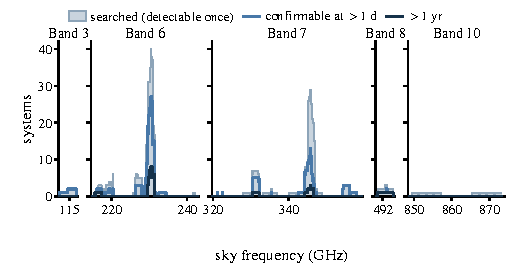
\includegraphics[width=\columnwidth]{figures/confcoverage.pdf}
\caption{What could be searched against what could be confirmed. For the
Class~A experiment, against sky frequency: the number of systems toward which
a carrier could have been detected once (grey), the number for which a block
of another observing session more than a day later also covers that frequency
(blue), and the same beyond a year (dark). Counted over the primary census; the
repeat blocks beyond it that \S\ref{sec:etacrv} reads add \ZcAddSupDayMHz\,MHz
to this support and move no curve visibly. One panel per populated ALMA band,
widths in proportion to the frequency each contributes, as in
Fig.~\ref{fig:covmap}.}
\label{fig:confcov}
\end{figure}

\subsection{The search space this archive opens}
\label{sec:newspace}

The searches of \citet{Steffes1994} and \citet{Mauersberger1996} reached
nearby stars above about 30\,GHz at one frequency only, and the one other
millimetre search of more than a single line, \citet{Mason2025},
covered \MasonBandMHz\,MHz of Band~3 toward far more distant stars
(\S\ref{sec:background}); Band~3 is searched here, in
\NWinBandThree{} windows down to \SurvFreqLo\,GHz including
$\beta$~Pictoris' CO $J=1\!-\!0$ control. The haystack axis of \citet{Wright2018} runs from \SttHayLoMHz\,MHz to
\SttHayHiGHz\,GHz, and this experiment covers \SttHayGHz\,GHz of it. Only
\SttHayFineGHz\,GHz of that is carrier search, because the Class~A union
spans \SurvFreqLoA--\SurvFreqHiA\,GHz, and the rest lies above the axis
altogether.

Union bandwidth overstates what that buys: different frequencies were searched
toward different numbers of stars and to very different
limits. Figure~\ref{fig:covmap} gives instead the number of independent systems
that would have yielded a recovery at ninety per cent completeness, against sky
frequency and transmitter power. At an EIRP of $\CovEirpRefTex$\,W the covered frequency falls to
\CovUnionAtRef\,GHz, which is \CovFracAtRef{} per cent of the union. It
reaches \CovNSysAtRef{} systems, and \CovNMaxAtRef{} at the best-covered
frequency near \CovNuMaxAtRef\,GHz. With no limit on power at all that
frequency reaches \CovNMaxFull{} of the \NSysClassA{} systems, and half the
sample is reached only above $\CovEirpHalf$\,W.

\begin{figure}
\centering
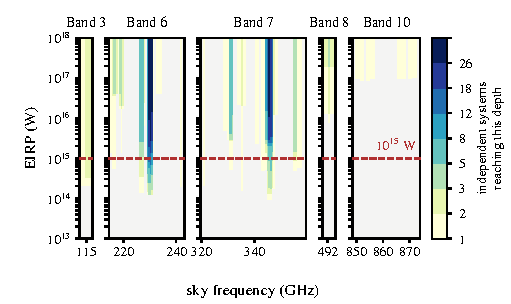
\includegraphics[width=\columnwidth]{figures/completeness_map.pdf}
\caption{Where the experiment could have found something. Shading gives the
number of independent systems in which an unresolved carrier of the plotted
EIRP at the plotted sky frequency would have been recovered nine times in
ten \emph{in a single epoch}; unshaded means none. That is a recovery
completeness and not a probability of confirmation: confirmation requires a
second independent epoch covering the same cell, which
Figure~\ref{fig:confcov} maps and which no amount of transmitted power can
supply. One panel per populated ALMA band, with panel widths in proportion
to the frequency each contributes: the \CvUnionA\,GHz Class~A union is
\CovNIslands{} disjoint islands across \DomAFreqLo--\DomAFreqHi\,GHz, which
a continuous abscissa would draw as hairlines. The dashed line is
$\CovEirpRefTex$\,W.}
\label{fig:covmap}
\end{figure}

The conventional measure for comparing programmes is the continuous-waveform
transmitter figure of merit of \citet{Enriquez2017},
$\mathrm{CWTFM}=\zeta_{\rm AO}\,\mathrm{EIRP}_{\rm min}/
(N_{\star}\nu_{\rm rel})$ with $\nu_{\rm rel}=\Delta\nu/\nu_{\rm mid}$,
smaller being better. Those programmes quote $\mathrm{EIRP}_{\rm min}$ at their own detection
thresholds, and the measure is linear in it. Put on the common footing of
five (Table~\ref{tab:litthresh}), \FomLitEnriquez{} becomes
\FomLitEnriquezFive{} and \FgLitMargot{} becomes \FgLitMargotFive. That runs
against this survey, making the comparison programmes deeper than their own
papers report -- on one arithmetic convention and not
at a matched false-alarm probability. \citet{Margot2023} publish no
CWTFM; the value quoted here is the same expression on the three quantities
they do give -- \FomMargotN{} stars, \FomMargotLo--\FomMargotHi\,GHz and
$\mathrm{EIRP}>\FgMargotEirp$\,W. This experiment takes no such factor. The
denominator used here modifies theirs: in place of a single survey-wide
fractional bandwidth it is the star-bandwidth product
$\sum_{i}\Delta\nu_{i}/\nu_{i}$, one term per system, in which
$\Delta\nu_{i}$ is the union of that system's own searched windows and
$\nu_{i}$ the midpoint of the span those windows cover. That is not the frequency of its best window, which is
what Table~\ref{tab:persys} lists; formed with those the same sum is
\CwSigmaBest, and the smaller of the two is adopted. The two are one quantity
for a survey in which every star is observed over the same band, which the
programmes compared here are, while for an archive a single fractional
bandwidth credits every system with frequencies searched toward another. Measured term by term it is \CwSigma{} over the \CwNSys{} systems, against
\CwUniform{} on the uniform convention. That factor of \CwRatio{} is there
because the median system was covered over only \SysUnionAMed\,GHz of the
\CvUnionA\,GHz union. On that denominator the Class~A experiment is
$\CwBareWorst$ on the sample's largest threshold power and $\CwBareMed$ on
the median system. On the $\mathrm{EIRP}_{90}$ adopted everywhere else here
it is $\CwAdoptWorst$ and $\CwAdoptMed$, a factor $\CwRatioEnriquez$ above
the published Enriquez value, widening to $\CwRatioEnriquezFive$ once that
value is put on the common threshold. That
gap is \CwBandDex{} decades of haystack and \CwEirpDex{} decades of depth, so
neither explains it alone: this is a far smaller haystack than a wideband
centimetre survey of thousands of stars and a shallower one, and the measure
compares surveys rather than estimating occurrence rates.

\subsection{What this experiment excludes, and what it does not}
\label{sec:excludes}

\noindent\emph{The signal these limits describe.} Every limit here applies to
one kind of signal: an unresolved carrier at the stellar position, confined to
a single \ChanLoA--\ChanHiA\,kHz channel, lying outside the molecular-line
mask, radiating while one of the archival blocks is on sky, and changing
frequency linearly at no more than its own window's ceiling,
\DriftCeilLo--\DriftCeilHi\,nHz. Such a carrier would
have produced a crossing nine times in ten above the nominal
$\mathrm{EIRP}_{90}$ of \S\ref{sec:pninetysel}, which excludes atmospheric
decorrelation, and none survived toward any of the \NSysClassA{}
systems the carrier search covers. Four conditions
bound it as sharply as power does: the coverage is sparse and
inherited (Fig.~\ref{fig:covmap}); the drift grid reaches an acceleration that contains every
known planet of the sample but one, while a transmitter on a rapidly rotating
planet spends most of that reach on its spin alone (Fig.~\ref{fig:accel}); emission broader than one channel is
removed with the spectral baseline; and a carrier on for part of a block comes
back at that fraction of its amplitude, while one absent throughout is not
constrained at all.

\noindent\emph{Recurrence applies over a far smaller domain.} Where the
archive observed a frequency only once, no transmitted power makes a
confirmation possible (\S\ref{sec:confirmability}). Where the test does apply
it has power only against a carrier as strong as the trigger demands of the
repeat, so a shallow repeat excludes nothing (\S\ref{sec:etacrv}).

\noindent\emph{The result is a non-detection and not an exclusion of
persistent transmitters.} An exclusion is read at the one cell the first
epoch predicts, so the transmitter it tests is one that comes back to that
cell, and four restrictions on that model are
ours. A transmitter operating intermittently need not have been radiating
during the second block. A second block need not cover the frequency at all,
and over about half the searched bandwidth none does
(\S\ref{sec:mmdifferent}). The interval that cell permits is half a channel in the star's own frame,
which the drifts fitted to these crossings cross in seconds
(\S\ref{sec:etacrv}), so a transmitter accelerating like that is in the
predicted cell again only if its motion is periodic and the second epoch
catches it at the matching phase. Anything else is left to the wide search
over the whole covering window at every drift. A transmitter may also change frequency deliberately,
and nothing here addresses that. Outside the adopted criterion, then, nothing
is excluded: neither emission inside the
$\pm\MaskHalfKms$\,km\,s$^{-1}$ molecular-line mask at any strength, nor any
emission from the stars within 40\,pc that ALMA has not
observed, which is almost all of the \NGaiaCensus{} this volume holds.

\noindent\emph{An illustrative engineering benchmark.} Take a \BenchDiam\,m dish radiating \BenchPowerMW\,MW at
\BenchFreqGHz\,GHz with an aperture efficiency of \BenchEta. Its directive
gain is $G=\eta(\pi D\nu/c)^{2}=\BenchGain$, so its EIRP is
$\BenchEirp$\,W -- above the single-epoch crossing limit of \BenchNSysA{} of the
\NSysClassA{} Class~A systems. The same gain makes its beam
$\Omega=4\pi/G=\BmOmegaSr$\,sr, \BmArcsec{} arcsec across and illuminating
$\BmSkyFrac$ of the sky. EIRP is not transmitter power -- the same megawatt
radiated isotropically would be $10^{6}$\,W -- so these limits apply to
beamed transmitters whose beam contains the Solar System.

\noindent\emph{Two blind spots.} The search forms Stokes~$I$ as
$(\mathrm{XX}+\mathrm{YY})/2$, which retains the full intensity of a circularly polarised
carrier; what is lost is not sensitivity but the discrimination polarisation
would offer against unpolarised astrophysical emission, because ALMA's feeds
are linear and the circularity lies in the cross-hands, which this analysis
does not extract. And the frequency coverage is the archive's and not a
choice: the \SbPriorFreqGHz\,GHz positronium hyperfine line that
\citet{Steffes1994} and \citet{Mauersberger1996} observed lies in ALMA Band~5,
where this survey holds
\LnBFiveWin{} coarse-channel windows, all toward \LnBFiveStars, and none of
them covers it.

\subsection{What a dedicated ALMA technosignature experiment should do
differently}
\label{sec:future}

A purpose-built experiment on the same telescope would be far stronger, and
the changes it needs follow from the limitations above. \emph{Channelise
finely everywhere:} the \NCoarse{} coarse-channel windows cannot carry a
carrier search at all.
\emph{Choose the targets and the frequencies:} an archive weighted toward
dusty discs is the worst case for molecular-line confusion, the M~dwarfs that
dominate the nearby habitable-zone planet census are the least covered, and
windows placed deliberately away from the bright transitions would recover
most of the \MkMaskAGHz\,GHz of the \CvUnionA\,GHz Class~A union that the
mask costs -- all three are decisions a
proposal can simply reverse. \emph{Repeat the epochs on purpose, at the same
tuning:} two or three visits separated by days and by years turn a crossing
into a testable claim, and the separation is a scheduling constraint rather
than extra sensitivity; Fig.~\ref{fig:confcov} is what its absence costs.
\emph{Retain the visibilities:} rotating the phase centre to the star leaves a
genuine point source entirely in the real part of the visibility. That asks
whether the data contain a source \emph{where the star is}, which is a
stronger question than any rank
against neighbouring positions in an image.
